\documentclass[12pt]{article}
\usepackage[margin=1in]{geometry} 
\usepackage{amsmath,amsthm,amssymb,amsfonts}
\usepackage{graphicx,fancyhdr,algorithm,algorithmic}
\usepackage[space]{grffile}
\usepackage{titlesec}
\usepackage{multicol}
\usepackage{enumitem} 
\usepackage{tikz}
\usepackage{tikz-qtree}
\usetikzlibrary{arrows,automata}


\cfoot{\thepage}
\renewcommand{\headrulewidth}{0.4pt}
\renewcommand{\headwidth}{\textwidth}
\renewcommand{\footrulewidth}{0.4pt}


\theoremstyle{definition}
\newtheorem{problem}{Problem}
\newtheorem{claim}{Claim}
\newtheorem{definition}{Definition}
\newtheorem{theorem}{Theorem}
\newtheorem{lemma}{Lemma}
\newtheorem{observation}{Observation}
\newtheorem{question}{Problem}

\newenvironment{solution}{\bigskip\noindent{\it Solution.}  \ignorespaces}{\hfill\qed}

\usepackage{hyperref}
\hypersetup{
    colorlinks=true,
    linkcolor=blue,
    filecolor=magenta,      
    urlcolor=cyan,
}
\urlstyle{same}
\PassOptionsToPackage{hyphens}{url}
\newcommand{\homework}[6]{
   \pagestyle{myheadings}
   \thispagestyle{plain}
   \newpage
   \setcounter{page}{1}
   \noindent
   \begin{center}
   \framebox{
      \vbox{\vspace{2mm}
    \hbox to 6.28in { {\bf CS256:~Algorithm Design and Analysis \hfill #1} }
       \vspace{6mm}
       \hbox to 6.28in { {\Large \hfill #2 \normalsize{#3}  \hfill} }
       \vspace{6mm}
     \hbox to 6.28in { {\it Instructor: #4 \hfill Source: #5} }
   }
   }
   \end{center}
   \markboth{#1}{#1}
   \vspace*{4mm}
}

\begin{document}
\homework{Spring 2021}{Recurrences Handout}{}{Shikha Singh}{\href{https://www.overleaf.com/read/vnkwvxbdfncg}{Overleaf}}



In this handout, we will look at examples of how to solve different recurrences using the recursion tree method.
 We look at three examples that each correspond to the three cases we discussed in class:  increasing series, decreasing series, and series with equal terms.
  

\begin{enumerate}[label = (\alph*)]
    \item\label{1a} $T(n) = 2T(n/2) + n^2$
    
     The recursion tree for this recurrence is given in Figure~\ref{rectree1}. Notice that the cost at each level is decreasing by at least a constant factor.
     The total cost at the root is $n^2$, one level down is $n^2/2$, and two levels down is $n^4/4$.
     In particular we get the following decaying geometric series $T(n) = n^2 (1 + 1/2 + 1/4 + \ldots) = \Theta(n^2)$.
     This falls into the first category of the recursion-tree method and the cost is dominant at the root, that is, $T(n) = O(n^2)$.
    \begin{figure}[h]
    \vspace{-5pt} 
    \centering
    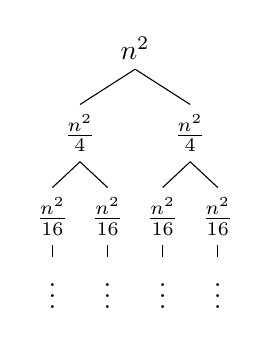
\begin{tikzpicture}
      %this package is useful for quickly making nice-looking trees
      %whitespace is unimportant: [ makes a new tree node; ] completes the node
    \Tree [.$n^2$ 
            [.${\frac{n^2}{4}}$ 
              [.${\frac{n^2}{16}}$ $\vdots$ ] 
              [.${\frac{n^2}{16}}$ $\vdots$ ] 
            ] 
            [.${\frac{n^2}{4}}$ 
              [.${\frac{n^2}{16}}$ $\vdots$ ] 
              [.${\frac{n^2}{16}}$ $\vdots$ ] 
            ] 
          ]
    \end{tikzpicture}\caption{Recursion Tree for \ref{1a}}\label{rectree1}
    \end{figure}   
    \vspace{-5pt} 


     
    \item\label{1b} $T(n) = 3T(n/2) + O(n)$
    
    
     The recursion tree for this recurrence is given in Figure~\ref{rectree2}. 

     The total cost at the root is $cn$, one level down is $3cn/2$, and two levels down is $9 cn/4$.
     We can conclude that the cost at each level is increasing by at least a constant factor, and must be asymptotically denominated by the leaves of the trees.  The number of leaves is $O(r^L)$ where $r$ is the branching factor and $L$ is the height of the tree.  The height of this tree is $L = \log_2 n$ (as problem size is going down by a factor 2 each time) and the branching factor is $r = 3$.  Thus, $T(n) = O(3^{\log_2 n}) = O(n^{\log_2 3})$.
    \begin{figure}[H]
    \vspace{-5pt} 
    \centering
    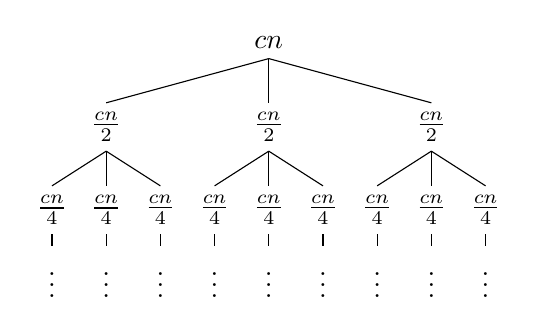
\begin{tikzpicture}
      %this package is useful for quickly making nice-looking trees
      %whitespace is unimportant: [ makes a new tree node; ] completes the node
    \Tree [.$cn$ 
            [.${\frac{cn}{2}}$ 
              [.${\frac{cn}{4}}$ $\vdots$ ] 
              [.${\frac{cn}{4}}$ $\vdots$ ] 
              [.${\frac{cn}{4}}$ $\vdots$ ] 
            ] 
            [.${\frac{cn}{2}}$ 
              [.${\frac{cn}{4}}$ $\vdots$ ] 
              [.${\frac{cn}{4}}$ $\vdots$ ] 
              [.${\frac{cn}{4}}$ $\vdots$ ] 
            ] 
          [.${\frac{cn}{2}}$ 
              [.${\frac{cn}{4}}$ $\vdots$ ] 
              [.${\frac{cn}{4}}$ $\vdots$ ] 
              [.${\frac{cn}{4}}$ $\vdots$ ] 
            ] 
          ]
    \end{tikzpicture}\caption{Recursion Tree for \ref{1b}}\label{rectree2}
    \end{figure}   
    \vspace{-5pt} 

  \item (Challenge) $T(n) = \sqrt{n} T(\sqrt{n}) + n$
  
  Notice that this recurrence does not quite fit into our mold of $T(n) = r T(n/c) + f(n)$, but that is okay.  We can still reason using a recursion tree and see what we get. 
  
  Actually, it is a bit hard to draw the recursion tree for this recurrence, but we can visualize it using words.  The root of the recursion tree does work $n$. The level below the root has $\sqrt{n}$ nodes, where each do work $\sqrt{n}$, with a total cost of $n$ again.  The level below we have $n^{1/4} \cdot n^{1/2}$ nodes, where each do work $n^{1/4}$, with a total work of $n$.  Thus, each level of the tree does exactly the same amount of work: $n$, so to figure out the overall cost, we have to determine the number levels (the height) of the tree.  Let us look at how the problem size is going down.  We have the following pattern 
  \[n \rightarrow n^{1/2} \rightarrow n^{1/4} \rightarrow n^{1/8} \rightarrow \ldots n^{1/2^i} \ldots\]
  
  We want to know when (at which level) this series gown down to a small number, say $2$.  Let us find that out by setting them equal and taking logs.  
  
  \begin{align*}
      n^{1/2^i} &= 2\\
      \frac{1}{2^i} \log_2 n &= 1\\
      \log_2 n &= 2^i\\
      \log_2 (\log_2 n) = i 
  \end{align*}
  
  Thus, the height of the tree is $\log\log n$ and the total cost is $T(n) = O(n \log \log n)$.
  
  \item Finally, to draw the connection between recursive algorithms and recurrences, we explain in words what an example recursive algorithm does and write its recurrence.
  
  Consider an algorithm that solves a problem of size $n$ by recursively solving two subproblems of half the size and combining their solutions in constant time.  The recurrence of this algorithm would be $T(n) = 2T(n/2) + O(1)$. What does this solve to?
  

\end{enumerate}

\end{document}


